\section{Business Logic Layer}
\subsection{Class Diagrams}


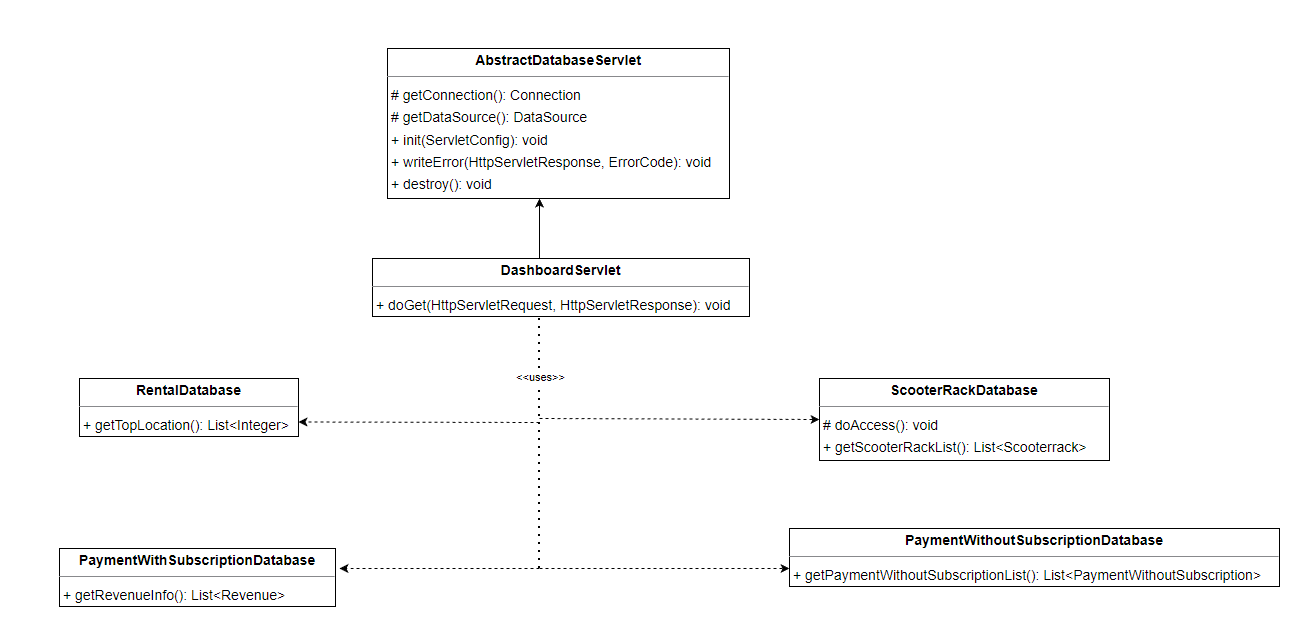
\includegraphics[scale=0.5]{sections/DLL/dashboard-servlet_CD.png}
This servlet uses the classes shown to access the database. This class diagram represents the classes involved in the dashboard servlet, which manages the dashboard page, it contains (some of) the classes used to handle three types of resources:scooter-Rack-List, top location, and revenue info. We used the proper queries to retrieve the necessary lists for each of these needed sections. For this, we used JDBC to establish a connection to the PostgreSQL database and ran the necessary queries from there. The desired tables were extracted, and the extracted queries were then turned into Java objects, and we used the proper queries to return the necessary lists for each of these desired sections. To achieve this, we used JDBC to establish a connection to the PostgreSQL database and ran the necessary queries. To present the collected data to the user, we had to extract from the relevant tables, turn the extracted queries into Java objects, and use JSP and HttpServlet technologies. 

As a result, we developed a servlet called dashboard servlet, and called the resources we already had, turned them into the appropriate Java models, then sent the desired characteristics to the page using the HttpServlet's APIs. We transferred the Jsp there and showed it, along with the following descriptions of the aforementioned sections.

\begin{enumerate}
    \item \textbf{scooterRackList}: shows a list of all locations where scooter rentals are available.
    \item \textbf{revenueInfo}: this shows the overall amount of money we made from renting scooters and our monthly income from scooter rentals.
    \item \textbf{top location}: using this reasoning, we can identify the city's busiest scooter rental location.
\end{enumerate}

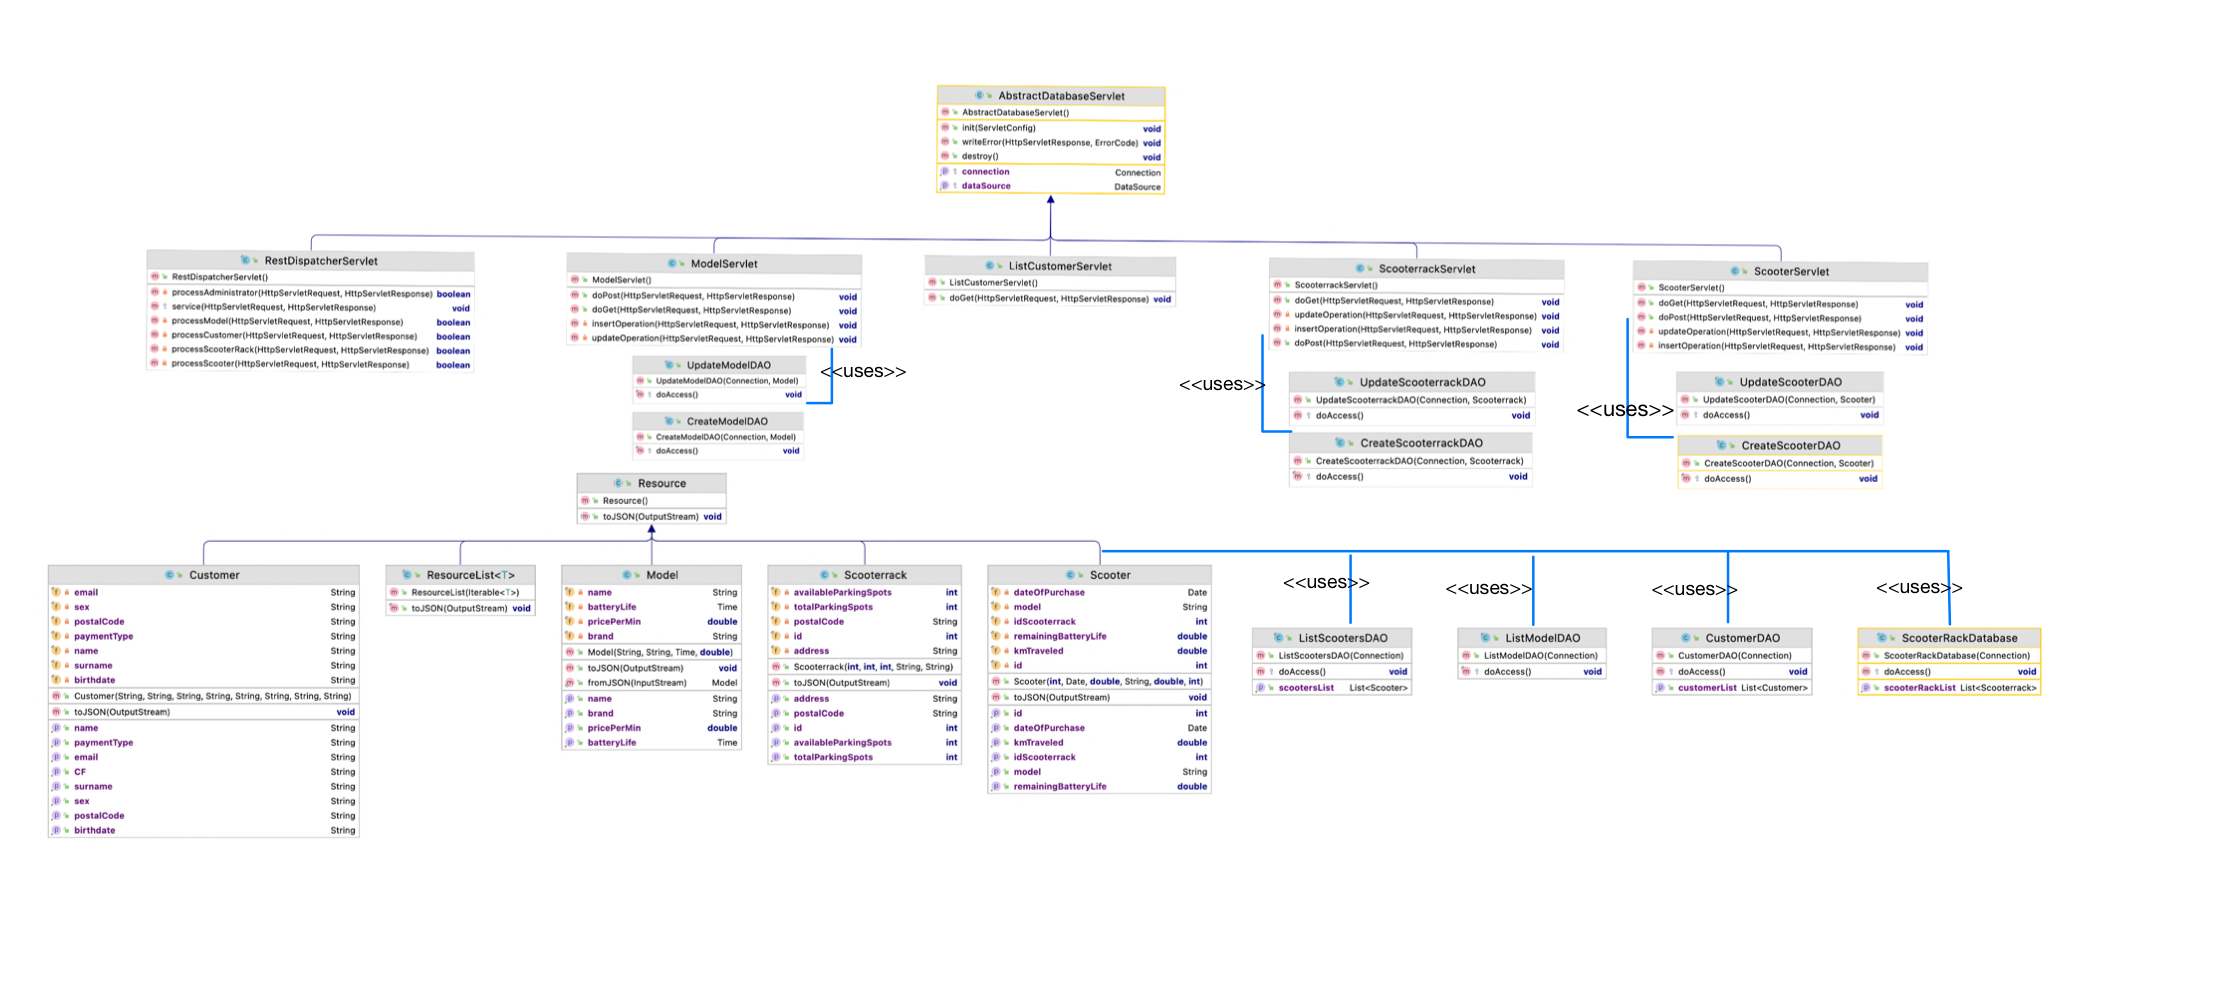
\includegraphics[scale=0.25]{sections/DLL/manage-servlet-rest.jpeg}

The second diagram represent the manage pages servlet and rest. The manage pages are model, scooter, scooter rack, rental, payment methods, customer and subscription. On these pages, we can interact with the respective tables of the database, for example: to view the list and add or edit that entity. In this case, we show the scooter, scooterracks, model and customer entities and have a servlet for viewing the list of scooters, one for adding a new scooter and one for editing an existing scooter. Then we also provide the REST API for getting the list of these entites. Both the rest and the servlets use some classes to access the database, as shown in the diagram. 
\subsection{Sequence Diagram}

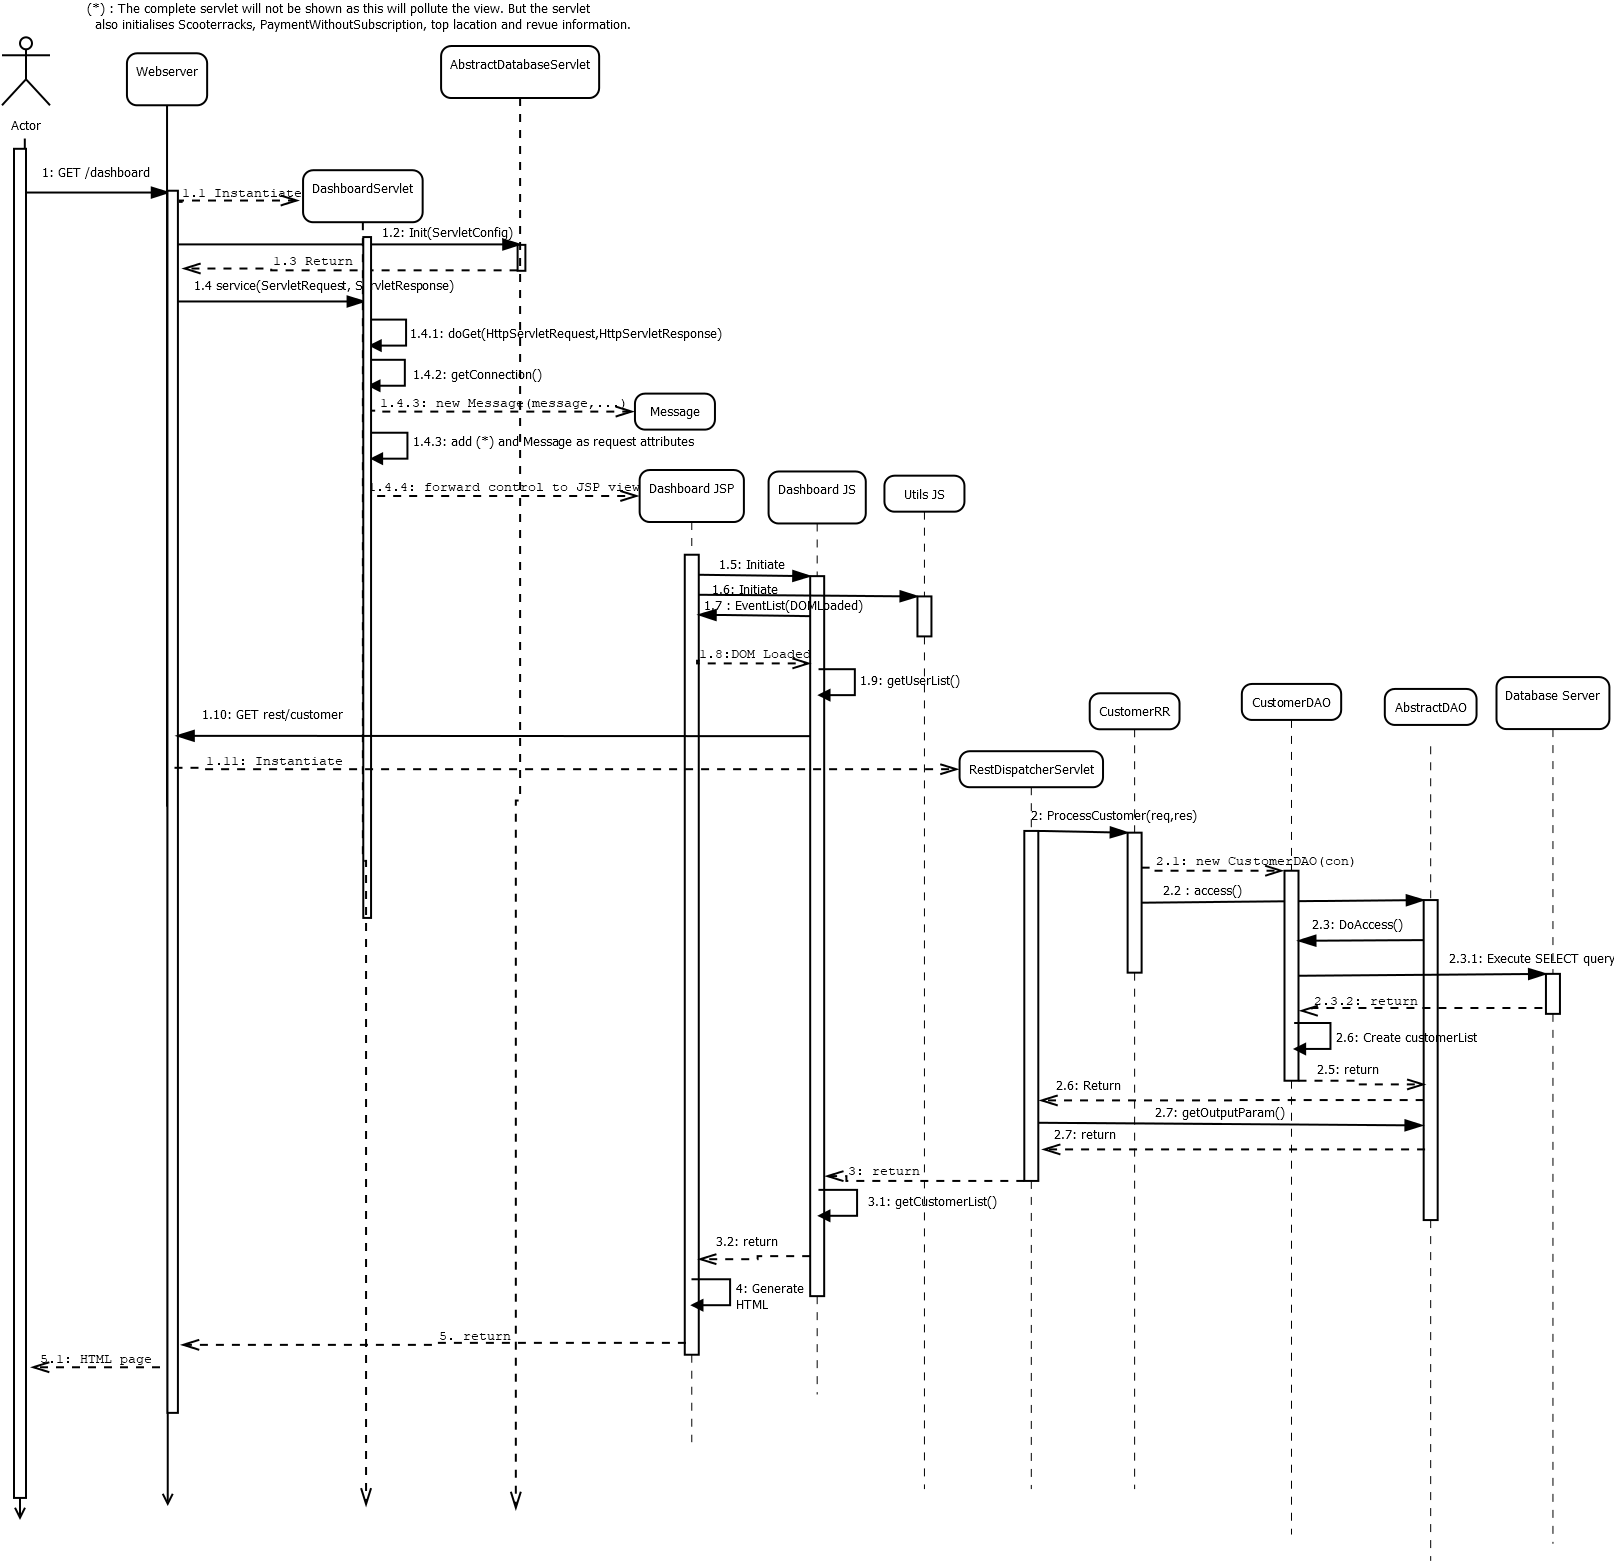
\includegraphics[scale=0.30]{sections/DLL/SequenceDiagramCustomerRestCall.png}

%describe here the sequence diagram
This sequence diagram depicts the communication flow for a REST API call from a JSP page (Dashboard) in our web application. The objective of this diagram is to illustrate the specific steps involved in the communication flow between the different components involved in this process.

\vspace{10pt} 

At the start of the sequence, an actor sends a request to the WebServer for the Dashboard page. The WebServer forwards this request to the DashboardServlet, which in turn renders the DashBoardJSP page. The DashBoardJSP page loads the necessary DashBoardJS script, which makes a HTTP GET request for retrieving customer data from the REST API (/rest/customer).

\vspace{10pt} 

The RestDispatcherServlet, which is responsible for handling all REST API requests in the web application, delegates the handling of the request to the CustomerRR class, which interacts with the CustomerDAO class to retrieve the customer data from the database. The customer data return to the CustomerRR object, which returns it to the RestDispatcherServlet. The RestDispatcherServlet then sends the response back to the dashboard js call, which in turn passes it to the last function (getCustomerList) which updates the HTML page.  

\vspace{10pt} 

Overall, this sequence diagram shows the complex interaction between different components involved in a REST API call in our web application, and how each component plays a specific role in this process. It was challenging to comprehend this communication flow, and this diagram helps to provide a visual representation of how the different components work together to retrieve and display data from the REST API.



\subsection{REST API Summary}


%describe the REST API. If needed, add a few lines of text here, describing the content of the table.
\caption{ The list of the rest API for this homweork are still "in progress" because we have to decide according to the frontend where it is better to use a REST call or not. There are some resources we used for rest in the next table.}

\begin{longtable}{|p{.375\columnwidth}|p{.1\columnwidth} |p{.35\columnwidth}|p{.1\columnwidth}|} 
\hline
\textbf{URI} & \textbf{Method} & \textbf{Description}  \\\hline
rest/scooter & GET &  Returns the list of scooters available in the database \\\hline
rest/scooterrack & GET & Returns the list of scooterracks available in the database \\\hline
rest/model & GET & returns the list of models available in the database \\\hline  
rest/customer & GET & returns the list of customers available in the database \\\hline

rest/administrator/id/\{id\} & GET & Returns the ID of the administrator from the database\\\hline
%rest/administrator/id & POST & Allows to insert the ID of the new administrator into the database \\\hline
%rest/administrator/id & DELETE & Allows to delete the ID of the administrator from the database \\\hline
%rest/administrator/id & PUT & Allows to update the list of administrators in the database \\\hline


rest/administrator/email/\{email\} & GET & Returns the Email of the administrator from the database\\\hline
%rest/administrator/email & POST & Allows inserting the Email-ID of the new administrator into the database \\\hline
%rest/administrator/email & DELETE & Allows deleting the Email-ID of the administrator from the database \\\hline
%rest/administrator/email & PUT & Allows updating the list of administrators in the database \\\hline



%rest/administrator & GET & Returns the administrator from the database\\\hline
%rest/administrator & POST & Allows to insert  the new administrator into the database \\\hline
%rest/administrator & DELETE & Allows to delete the administrator from the database \\\hline
%rest/administrator & PUT & Allows to update the list of administrators in the database \\\hline



%administrator/password & GET & Returns the password of the //administrator from the database\\\hline
%administrator/password & POST & Allows inserting the password of the new administrator into the database \\\hline
%administrator/password & DELETE & Allows deleting the password of the administrator from the database \\\hline
%administrator/password & PUT & Allows updating the list of administrators in the database \\\hline


\end{longtable}
\subsection{REST Error Codes}

%If needed, add few lines of text, describing the error codes table
Here is the list of errors defined in the application.


\begin{longtable}{|p{.15\columnwidth}|p{.2\columnwidth} |p{.6\columnwidth}|} 
\hline
\textbf{Error Code} & \textbf{HTTP Status Code} & \textbf{Description} \\\hline

-103 & BAD\_REQUEST &   missing Email\\\hline
-104 & BAD\_REQUEST &   missing Password \\\hline
-105 & BAD\_REQUEST &  Submitted credentials are wrong \\\hline
-200 & BAD\_REQUEST &  Operation unknown \\\hline
-999 & INTERNAL\_SERVER
\_ERROR &  Internal Error \\\hline
-E100 &  &  cannot search for the rentals in the database\\\hline
-E200 &  &  cannot search for the rentals: unexpected error while accessing the database\\\hline
-E300 &   & cannot create the administrator: administrator already exists\\\hline
-E400 &  &  unsupported multimedia type for an employee photo. expected image/png or image/jpg\\\hline
-E4A1 & BAD\_REQUEST &  Accept request header missing\\\hline
-E4A2 & NOT\_ACCEPTABLE &  unsupported output media type. resources are represented only in application/json\\\hline
-E4A3 & BAD\_REQUEST &  Input media type not specified. content-type request header issing\\\hline
-E4A4 & BAD\_REQUEST &  unsupported input media type. resources are represented only in application/json.\\\hline
-E4A5 & METHOS\_NOT
\_ALLOWED  &  unsupported operation\\\hline
-E4A6 & NOT\_FOUND &  unknown resource requested\\\hline
-E4A7 & BAD\_REQUEST &  wrong format for URL, e.g.: /administrator/email/{email}: no {email} specified\\\hline
-E4A8 &  BAD\_REQUEST &  cannot create the resource, e.g.: no administrator JSON object found in the request\\\hline
-E5A1 & INTERNAL\_SERVER
\_ERROR   & Cannot create the resource: unexpected error.\\\hline
-E5A2 & CONFLICT  &  cannot create the resource. it already exists\\\hline
-E5A3 & NOT\_FOUND  &  resource Not found. cannot delete it.\\\hline
-E5A4 & CONFLICT &   cannot delete resource: other resources depend on it.\\\hline
-E10A1 & INTERNAL\_SERVER
\_ERROR &  cannot list resource: unexpected error
\\\hline


\caption{ REST API}
\label{tab:termGlossary}
\end{longtable}

\subsection{REST API Details}

%List here a few resources retrievable via REST API
We reported three different types of resources that our web applications handle.

\subsubsection*{ Available scooter's list in the database}
% the description of the resource
The following endpoint allows to a list getting all scooters which are available in the database.

\begin{itemize}
    \item URL: \texttt{ rest/scooters}
    \item Method: \texttt{GET}
    \item URL Parameters: No parameters are required in the URL
    \item Data Parameters: No parameters are required
    \item Success Response: Upon success, the servlet returns a JSON object with the required information.
    \item Error Response:
    
Code: INTERNAL\_SERVER\_ERROR \newline
Content:‘‘code’’: -E5A1, \{‘‘message’’ :\{‘Cannot list scooter(s): unexpected database error.'\}\} \\
Code: INTERNAL\_SERVER\_ERROR \newline
Content:‘‘code’’: -E5A1, \{‘‘message’’ :\{'Cannot list scooter(s): unexpected error.'\}\}
    
\end{itemize}

\subsubsection*{ Available scooter rack's list in the database}
% the description of the resource
The following endpoint allows to a list getting all scooter racks which are available in the database.

\begin{itemize}
    \item URL: \texttt{ rest/scooterrack}
    \item Method: \texttt{GET}
    \item URL Parameters: No parameters are required in the URL
    \item Data Parameters: No data parameters required.
    \item Success Response: Upon success, the servlet returns a JSON object with the required information.
    \item Error Response:
Code: INTERNAL\_SERVER\_ERROR \newline
Content:‘‘code’’: -E5A1, \{‘‘message’’ :\{‘Cannot list employee(s): unexpected database error.'\}\} \\
Code: INTERNAL\_SERVER\_ERROR \newline
Content:‘‘code’’: -E5A1, \{‘‘message’’ :\{'Cannot list employee(s): unexpected error.'\}\}
    
\end{itemize}

\subsubsection*{ Scooter model's list in the database}
% the description of the resource
The following endpoint allows to a list getting all scooter models in the database.

\begin{itemize}
    \item URL: \texttt{ rest/model}
    \item Method: \texttt{GET}
    \item URL Parameters: No parameters are required in the URL
    \item Data Parameters: No data parameters required.
    \item Success Response: Upon success, the servlet returns a JSON object with the required information.
    \item Error Response: 

Code: INTERNAL\_SERVER\_ERROR \newline
Content:‘‘code’’: -E6A1, \{‘‘message’’ :\{‘Cannot list models: unexpected error'\}\}
\\
Code: INTERNAL\_SERVER\_ERROR \newline
Content:‘‘code’’: -E6A2, \{‘‘message’’ :\{'Cannot search models: unexpected error.'\}\}
    
\end{itemize}


\subsubsection*{Customer's list in the database}

\begin{itemize}
    \item URL: \texttt{ rest/customer}
    \item Method: \texttt{GET}
    \item URL Parameters: No parameters are required in the URL
    \item Data Parameters: No data parameters required.
    \item Success Response: Upon success, the servlet returns a JSON object with the required information.
    \item Error Response:
    
Code: INTERNAL\_SERVER\_ERROR \newline
Content:‘‘code’’: -E10A1, \{‘‘message’’ :\{‘Cannot list customer(s): unexpected database error.'\}\}
\\
Code: INTERNAL\_SERVER\_ERROR \newline
Content:‘‘code’’: -E10A1, \{‘‘message’’ :\{'Cannot list customer(s): unexpected error.'\}\}
\end{itemize}


\subsubsection*{ Administrator- ID }
the following endpoint allows the access of the inf 
\begin{itemize}
    \item URL: \texttt{ rest/administrator/id/\{id\}}
    \item Method: POST
    \item URL Parameters: Required: administrator ID: the identifier of the administrator.
    \item Data Parameters: 
    \begin{itemize}
       \item  Id:\{int\}
    \end{itemize}
    \item Success Response: Upon success, the servlet returns a JSON object with the required information.
        \begin{itemize}
       \item  Id:\{int\}
       \item  email:\{string\}
       \item  password:\{string\}
    \end{itemize}

    Content:"administrator":\{"id":1,"email":"admin@wascoot.com","password":"123321"\}\}
    \item Error Response: 
     
Code: INTERNAL\_SERVER\_ERROR \newline
Content:‘‘code’’: -E5A1, \{‘‘message’’ :\{‘Cannot search administrator(s): unexpected database error.'\}\}
\\
Code: BAD\_REQUEST\newline
Content:‘‘code’’: -E4A7, \{‘‘message’’ :\{'Cannot search administrator(s): wrong format for URI /administrator/id/{id}.'\}\}
\\
Code: INTERNAL\_SERVER\_ERROR\newline
Content:‘‘code’’: -E5A1, \{‘‘message’’ :\{'Cannot search administrator(s): unexpected error.'\}\}
    
\end{itemize}

\subsubsection*{ Administrator- Email }

\begin{itemize}
    \item URL: \texttt{ rest/administrator/email/\{email\}}
    \item Method: POST
    \item URL Parameters: Required: administrator email: the email of the administrator.
    \item Data Parameters: 
    \begin{itemize}
       \item  email:\{string\}
    \end{itemize}
    \item Success Response: Upon success, the servlet returns a JSON object with the required information.
    \begin{itemize}
       \item  Id:\{int\}
       \item  email:\{string\}
       \item  password:\{string\}
    \end{itemize}
    "administrator":\{"id":1,"email":"admin@wascoot.com","password":"123321"\}
    
    \item Error Response:
Code: INTERNAL\_SERVER\_ERROR \newline
Content:‘‘code’’: -E5A1, \{‘‘message’’ :\{‘Cannot search administrator(s): unexpected error.’\}\}
\\
Code: BAD\_REQUEST \newline
Content:‘‘code’’: -E4A7, \{‘‘message’’ :\
{‘Cannot search administrator(s): wrong format for 
URL/administrator/email/{email}.’\}\}
\\
Code: INTERNAL\_SERVER\_ERROR \newline
Content:‘‘code’’: -E5A1, \{‘‘message’’ :\{‘Cannot search administrator(s): unexpected database error’\}\}


\end{itemize}

